\section{State of the art}
\AtBeginSection[]
  {
     \begin{frame}<beamer>
     \frametitle{Plan}
     \tableofcontents[currentsection]
     \end{frame}
  }
\subsection{The simplex algorithm}

\begin{frame}{Linear optimization problems}
A linear optimization problem is to maximise a linear function under linear constrains (inequalities). The variables are positive and $0$ is in all the constrains. 

The constrains are in fact half-spaces.
\begin{example}

Maximize $x+y$ under $y\leq 2$ and $x-y\leq 2$.
\vspace*{-0.5cm}
\begin{figure}
%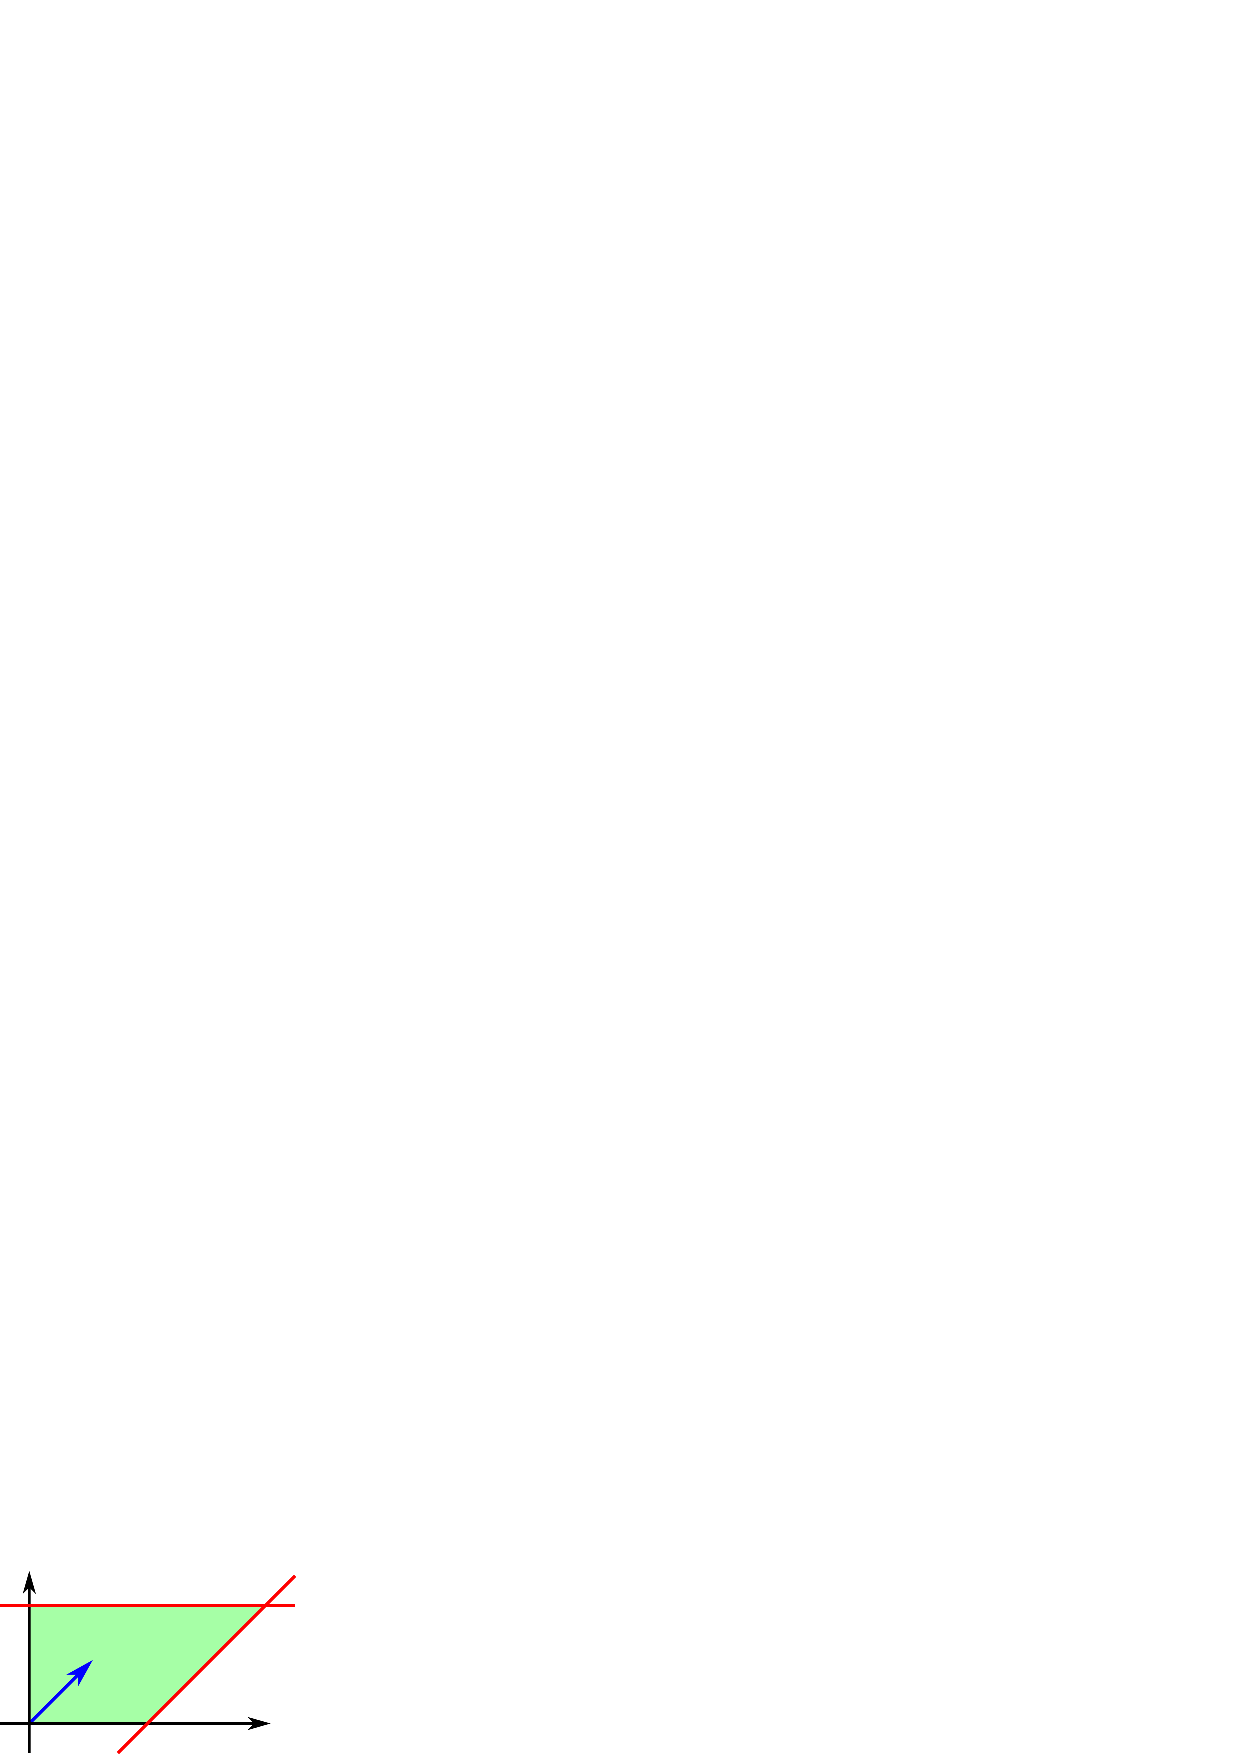
\includegraphics[scale=0.6]{images/simplex1.pdf}
\caption{Geometrical interpretation of the problem}
\end{figure}
\vspace*{-0.5cm}
\end{example}
The set of points that respect all the constrains is the feasible area. If a point is on a constrain, the constrain is saturated by the point (the constrain becomes an equality). 
\end{frame}

\begin{frame}{How to simplex}
\begin{theorem}
A vertex maximizes the objective.
\end{theorem}
The concept is to explore the vertices to find the optimal one.

To obtain a vertex: saturate $d$ constrains.

To obtain a new vertex: switch a saturated constrain for another one.

\begin{figure}
\only<1>{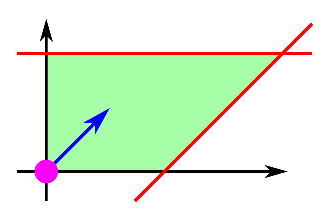
\includegraphics[scale=1]{images/simplex12.eps}}
\only<2>{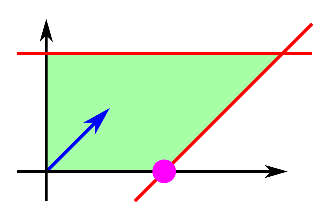
\includegraphics[scale=1]{images/simplex13.eps}}
\only<3>{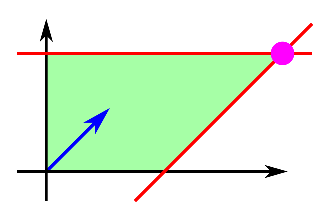
\includegraphics[scale=1]{images/simplex14.eps}}
\caption{The simplex on the previous example}
\end{figure}  

\end{frame}

\begin{frame}{The dictionary}
The magic of the simplex happens with a powerful tool: the dictionary.
A positive \emph{slack} variable is associated to each constrains. Setting a variable to $0$ saturates the constrain.
\begin{block}{Construction of the slack variables}
$-x+y\leq 3 \hspace*{1cm} \rightarrow \hspace*{1cm} 0 \leq x - y + 3 \hspace*{1cm} \rightarrow \hspace*{1cm} s_1 = x - y + 3$
\end{block}
The dictionary keeps track of all the constrains.
\begin{block}{Construction of the dictionary}
\begin{tabular}{| c  c  c  c  c | c c |}
	\hline	
   	$-x$ &$+$& $0$ & $+$ & $2$ & = & $s_1$\\ \hline	
   	$x$ &$+$& $-y$ & $+$ & $3$ & = & $s_2$\\ \hline \hline	
   	$x$ & $+$ & $y$ & & & &  \\
   	\hline	
\end{tabular}
$\rightarrow$
\begin{tabular}{| c | c || c || c c |}
	\hline	
	$x$ & $y$ & const & & \\
	$\downarrow$ &$\downarrow$ &$\downarrow$ & & \\
	\hline
	\hline	
   	$-1$ & $0$ & $2$ & = & $s_1$\\ \hline	
   	$1$ & $-1$ & $3$ & = & $s_2$\\ \hline \hline	
   	$1$ & $1$ & $0$ & $\leftarrow$ & obj \\
   	\hline	
\end{tabular}

\end{block}

\end{frame}

\begin{frame}{Some properties}
\begin{columns}[c]
\begin{column}{5cm}
\begin{tabular}{| c | c || c || c c |}
	\hline	
	$x$ & $y$ & const & & \\
	$\downarrow$ &$\downarrow$ &$\downarrow$ & & \\
	\hline
	\hline	
   	$-1$ & $0$ & $2$ & = & $s_1$\\ \hline	
   	$1$ & $-1$ & $3$ & = & $s_2$\\ \hline \hline	
   	$1$ & $1$ & $0$ & $\leftarrow$ & obj \\
   	\hline	
\end{tabular}
\end{column}
\begin{column}{5cm}
Two sets of variables:
\begin{itemize}
\item the cobasis, the variables in the columns;
\item the basis, the variables in the rows;
\end{itemize}
\end{column}
\end{columns}
\vspace*{0.5cm}
\begin{itemize}
\item The variables of the cobasis are sufficient to express the variables of the basis.
\item The variables of the cobasis are independent.
\item Setting the cobasis to $0$ gives a vertex. The dictionary describes the vertex.
\end{itemize}

Only one operation to modify the dictionary: the pivot, it permutes a variable in the cobasis with a variable in the basis.
\end{frame}

\begin{frame}{Other version of the simplex}
If there are non positive variables or if $0$ is not in the feasible area.
\begin{itemize}
\item For each variable, keep lower and upper bounds, plus a valuation.
\item While there is a basic variable out of it bounds, pivot with a variable that can increase/decrease and modify the assignment.
\item Optimize.
\end{itemize}

\begin{figure}

\includegraphics[scale=1]{images/simplex2.eps}
\caption{Example of the other version of the simplex with $y\leq 0$ and $x+y\leq -1$.}
\end{figure}
\end{frame}

\subsection{Fukuda's algorithm}

\begin{frame}{Fukuda's algorithm}
Enumerates the vertices of a bounded $H$-polyhedron. The origin must be a vertex and the vertices must be positive. 
\begin{block}{Main idea}
Consider $-\sum_{i=0}^d x_i$ as a cost function (the origin maximises the function for $\mathbb{R}^d$). From every vertex, the origin will be reach by a unique path, walking backward on these path allow to find them all.
\end{block}

\begin{itemize}
\item All the vertices are found.
\item If there exist several ways of defining a vertex, all the ways will be found. 
\item Using Bland's rule to walk on the paths ensures staying inside the feasible area.
\end{itemize}


\end{frame}

\begin{frame}{An example}
Fukuda's Algorithm with the constrain $ x+2y \leq 4 $.
\begin{columns}[c]
\begin{column}{5cm}
\only<1,3>{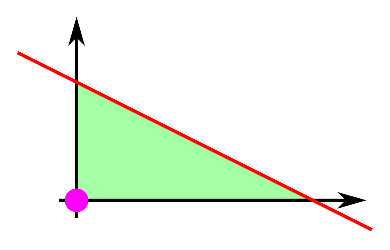
\includegraphics[scale=0.9]{images/fukuda0.eps}}
\only<2>{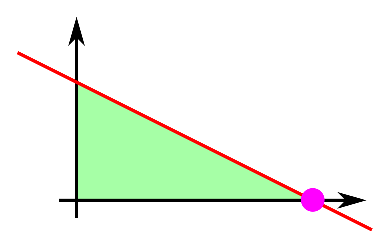
\includegraphics[scale=0.9]{images/fukuda1.eps}}
\only<4>{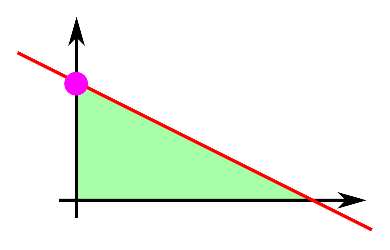
\includegraphics[scale=0.9]{images/fukuda2.eps}}
\end{column}
\begin{column}{5cm}
\begin{tabular}{| c | c || c || c c |}
	\hline	
	$x$ & $y$ & const & & \\
	$\downarrow$ &$\downarrow$ &$\downarrow$ & & \\
	\hline
	\hline	
   	$-1$ & $-2$ & $4$ & = & $s_1$\\ \hline \hline	
   	$-1$ & $-1$ & $0$ & $\leftarrow$ & obj \\
   	\hline	
\end{tabular}

\vspace*{0.3cm}

\only<2>{
\begin{tabular}{| c | c || c || c c |}
	\hline	
	$s_1$ & $y$ & const & & \\
	$\downarrow$ &$\downarrow$ &$\downarrow$ & & \\
	\hline
	\hline	
   	$-1$ & $-2$ & $4$ & = & $x$\\ \hline \hline	
   	$1$ & $1$ & $-4$ & $\leftarrow$ & obj \\
   	\hline	
\end{tabular}
}
\only<4>{
\begin{tabular}{| c | c || c || c c |}
	\hline	
	$x$ & $s_1$ & const & & \\
	$\downarrow$ &$\downarrow$ &$\downarrow$ & & \\
	\hline
	\hline	
   	$-\frac{1}{2}$ & $-\frac{1}{2}$ & $2$ & = & $y$\\ \hline \hline	
   	$-\frac{3}{2}$ & $\frac{1}{2}$ & $-2$ & $\leftarrow$ & obj \\
   	\hline	
\end{tabular}
}
\end{column}
\end{columns}
\end{frame}
